The grasping system proposed, shown in Figure \ref{fig:systemArchitecture}, consists of a learned generative model and an evaluative model. The generative model is a method that generates a number of candidate grasps given a point cloud, as explained in the previous section. An evaluative model is paired with a generative model in order to estimate a probability of success for each candidate grasp. EM1 and EM3 are VGG-16 based visual models, while EM2 is a modified ResNet-50 architecture. All evaluative models process the visual data and hand trajectory parameters in two separate pathways, and combine them to feed into a third processing block to produce the final success probability. In addition, we will present techniques for grasp optimisation using the EM as the objective function, using both Gradient Descent (GD) and Simulated Annealing (SA). Finally, we may train each model with either the data set of simulated grasps generated by GM1, by GM2, or by both combined. Table \ref{table:GEBreakdown} shows a the full list of 17 variants we test.

\begin{table}[]
\centering
\begin{tabular}{|l|l|l|l|l|l|l|}
\hline
Variant & GM/  & EM & Opt'  & Training Set \\ 
 & Testset & & Meth' & \\ \hline
V1 & GM1    & - & - & 10 grasps  \\ \hline
V2 & GM2    & - & - & 10 grasps  \\ \hline
V3 & GM1/DS1-Te & EM1 & - & DS1-Tr \\ \hline
V4 & GM1/DS1-Te & EM2 & - & DS1-Tr \\ \hline
V5 & GM1/DS1-Te & EM3 & - & DS1-Tr  \\ \hline
V6 & GM1/DS1-Te & EM1 & - & DS1-Tr + DS2-Tr \\ \hline
V7 & GM1/DS1-Te & EM2 & - & DS1-Tr + DS2-Tr \\ \hline
V8 & GM1/DS1-Te & EM3 & - & DS1-Tr + DS2-Tr \\ \hline
V9 & GM2/DS2-Te & EM1 & - & DS1-Tr + DS2-Tr \\ \hline
V10 & GM2/DS2-Te & EM2 & - & DS1-Tr + DS2-Tr \\ \hline
V11 & GM2/DS2-Te & EM3 & - & DS1-Tr + DS2-Tr \\ \hline
V12 & GM1/DS1-Te & EM3 & GD1 & DS1-Tr + DS2-Tr \\ \hline
V13 & GM1/DS1-Te & EM3 & GD2 & DS1-Tr + DS2-Tr \\ \hline
V14 & GM1/DS1-Te & EM3 & GD3 & DS1-Tr + DS2-Tr \\ \hline
V15 & GM1/DS1-Te & EM3 & SA1 & DS1-Tr + DS2-Tr \\ \hline
V16 & GM1/DS1-Te & EM3 & SA2 & DS1-Tr + DS2-Tr \\ \hline
V17 & GM1/DS1-Te & EM3 & SA3 & DS1-Tr + DS2-Tr \\ \hline
\end{tabular}
\caption{The evaluated combinations of architecture, generative model/test set, training set, and optimisation method (Gradient Descent (GD) or Stochastic Simulated Annealing (SA).}
\label{table:GEBreakdown}
\end{table}

In this section, the three proposed evaluative model (EM) architectures are explained. The grasp generator models, GM1 and GM2, given in the previous section, require very little training data to train, here being trained from 10 example grasps. %GM1 can generate 500 candidate grasps, ranked according to their estimated likelihoods, within 10 seconds on a 2x Intel Xeon E5-2650 v2 Eight Core 2.6GHz. GM2 takes a 50 seconds to create 250 grasps in the same setting. 
These generative models do not, however, estimate a probability of success for the generated grasps. An evaluative model, which is a Deep Neural Network (DNN), is used specifically for this purpose. DNNs have shown good performance in learning to evaluate grasps using two-finger grippers \cite{levine16,lenz2015deep}. They have also been applied to generating pre-grasps, so as to perform power grasps with dexterous hands \cite{varley2015generating,lu2017planning}.

%The generative approach ignores the global information about the object, such as overall shape and the object category. The success of an executed grasp, however, depends on many contextual factors such as full object shape, mass, mass distribution and surface friction. An evaluative network can indirectly learn to predict grasp success from image data. 
%The data provided to the evaluative network is collected from randomly generated scenes, therefore each scene has a different random combination of the parameters. The primary purpose of the network is to learn robust grasps across different conditions, and this is a complex task. The first challenge is that the kinematic model of the hand is unknown to the evaluative network. It only has access to the parameters that \textit{configure} the hand: the wrist and joint positions. Second, the system is weakly supervised with the grasp result (success or failure), and no further labels are provided.

We tested three evaluative models. The first is based on the VGG-16 network \cite{Simonyan14c}, named Evaluative Model 1 (EM1), and shown in Figure \ref{fig:networkArchitecture2} (a). A version based on the ResNet-50 network, termed EM2, is shown in Figure \ref{fig:networkArchitecture2} (b). Finally, EM3 (Figure \ref{fig:networkArchitecture2} (c) is also based on VGG-16. Regardless of the type, a grasp evaluation network has the functional form $f(I_t, h_t)$, where $I_t$ is a colourised depth image of the object, and $h_t$ contains a series of wrist poses and joint configurations for the hand, converted to the camera's frame of reference. The network's output layer calculates a probability of success for the image-grasp pair $I_t$, $h_t$. The model initially processes the grasp parameters and visual information in separate channels, and combines them to feed into a feedforward pipeline that produces the output. 

%\begin{figure}[h]
%  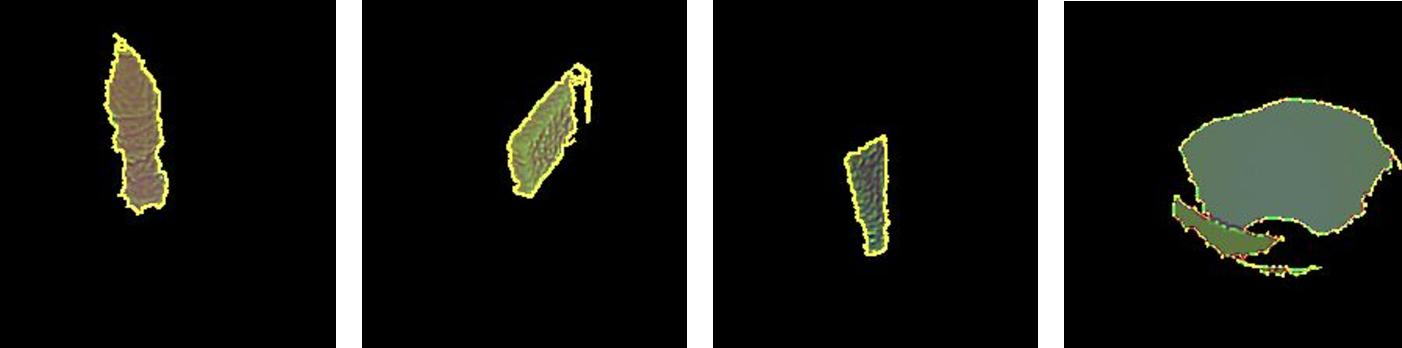
\includegraphics[width=0.9\linewidth]{images/colourDepth.pdf}
%  \caption[Colourised depth images.]{Colourised depth images. From left to right, the objects are: coke bottle, chocolate box, hand cream, and bowl.}
%\label{fig:colorisedDepth}
%\end{figure}

The depth image is colourised before it is passed as input to the evaluative network. The colourisation process converts the single-channel depth data to a 3-channel RGB image. We first crop the middle $460 \times 460$ section of the $640 \times 480$ depth image, and down-sample it to $224 \times 224$. Then, two more channels of the same dimension are added corresponding to the mean and Gaussian curvatures. Figure~\ref{fig:colorisedDepth} contains four examples of colourised depth images. This procedure both provides a meaningful set of depth features to the network, and makes the input compatible with VGG-16 and ResNet, which require images of size $224 \times 224 \times 3$.

The grasp parameter data $h_t$ consists of 10 trajectory waypoints represented by $27 \times 10 = 270$ floating point numbers, and 10 extra numbers reserved for the grasp type. Each of the 10 training grasps is treated as a different class, and $h_t$ uses the 1-of-N encoding system. Based on the grasp type ([1-10]), the corresponding entry is set to 1, while the rest remain 0. The grasp parameters are converted to the coordinate system of the camera which was used to obtain the corresponding depth image. In EM1 and EM2, the transformed parameters are processed using a fully-connected (FC) layer consisting of 1024 nodes, and the output is \textit{element-wise added} to the visual features. EM3 uses a convolutional approach instead. In all networks, the joint visual features and grasp parameter data are joined in higher layers.

All FC layers have RELU activation functions, except for the output layer, which uses 2-way softmax. The output layer has two nodes, corresponding to the success and failure probabilities of the grasp. A cross-entropy loss is used to train the neural network, as given in \eq\ref{equation:crossentropy}.

\begin{equation}
H_{y'}(y) := - \sum_{i} ({y_i' \log(y_i) + (1-y_i') \log (1-y_i)})
\label{equation:crossentropy}
\end{equation}
where $y_i'$ is the class label of the grasp, which is either 1 (success) or 0 (failure), and $y_i = f(I_i, h_i)$ is is the predicted label of the grasp pair ($I_i$, $h_i)$.

The proposed evaluative models EM1-3 share the common features explained above. The individual models are now introduced below. Only their unique properties are highlighted.

\begin{figure*}[t]
\centering
% \begin{center}
\subfloat[Evaluative Model 1]{%
  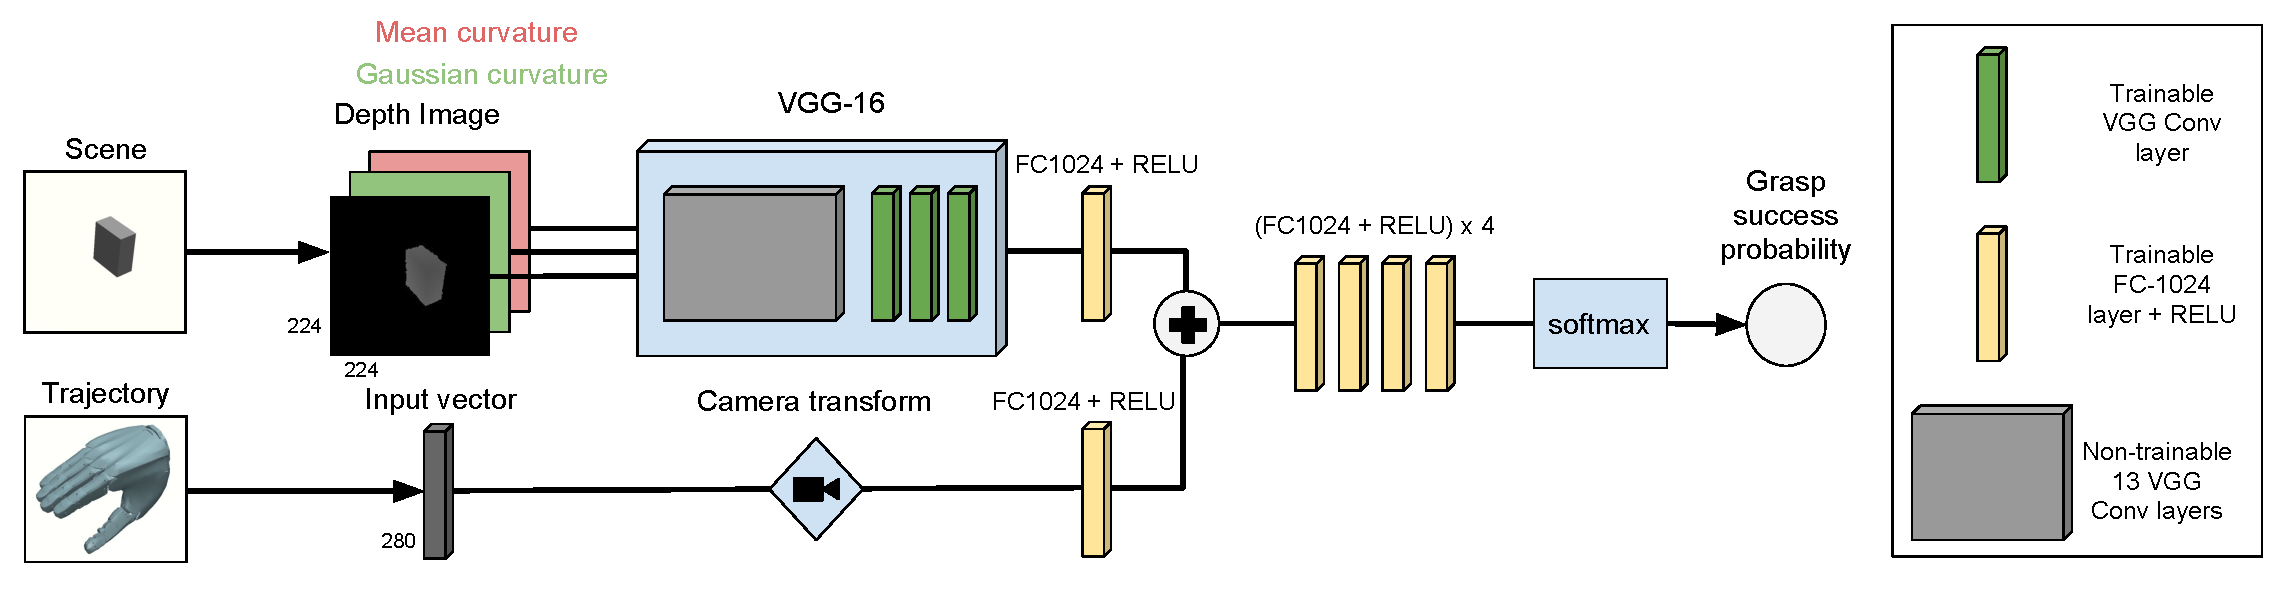
\includegraphics[width=0.9\textwidth]{images/networkArchitecture.pdf}
}
% \end{center}

% \begin{center}
\subfloat[Evaluative Model 2]{%
    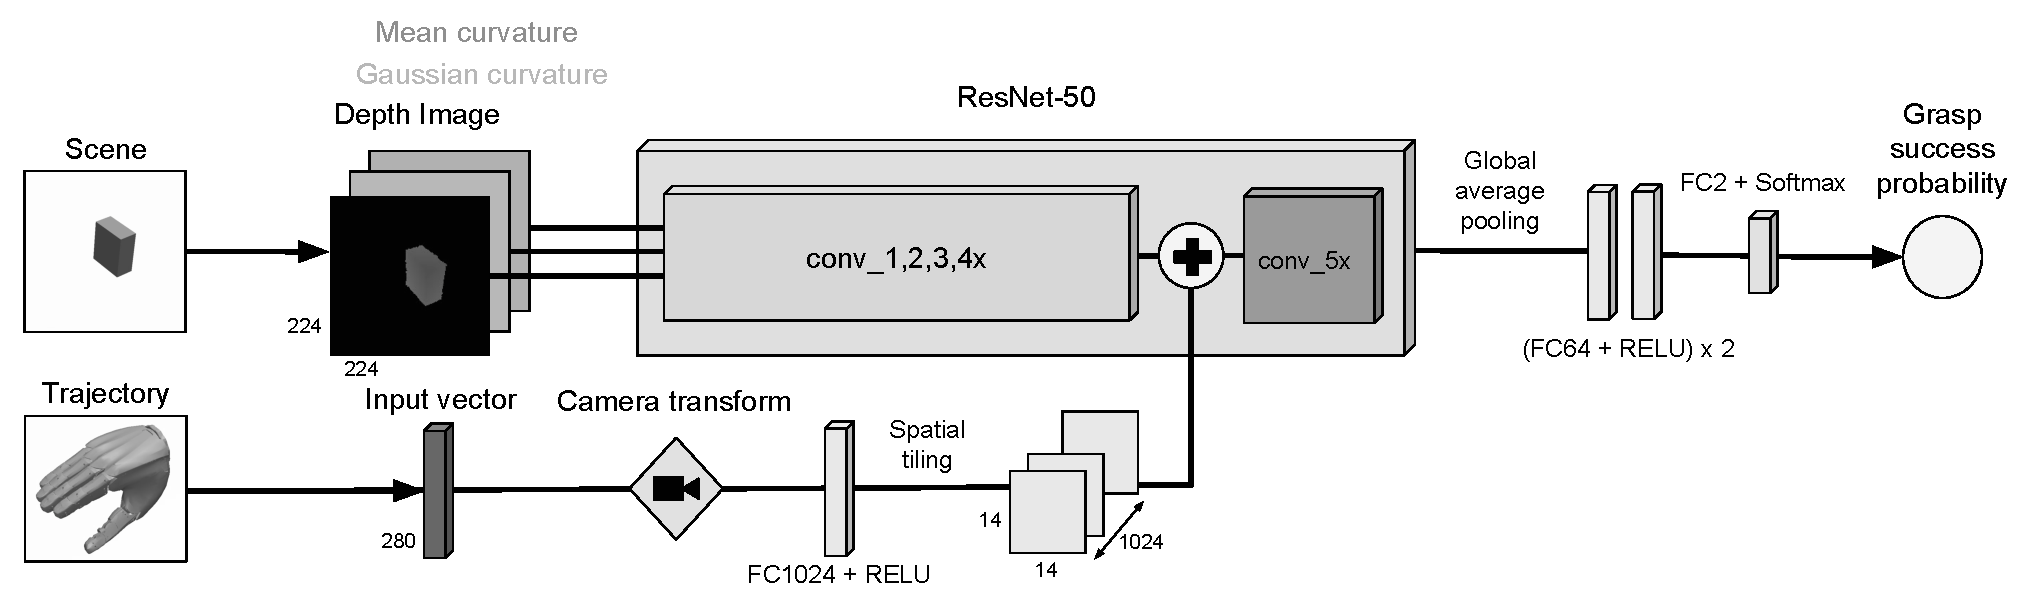
\includegraphics[width=0.8\textwidth]{images/ResNet.pdf}
}
% \end{center}

% \begin{center}
\subfloat[Evaluative Model 3]{%
    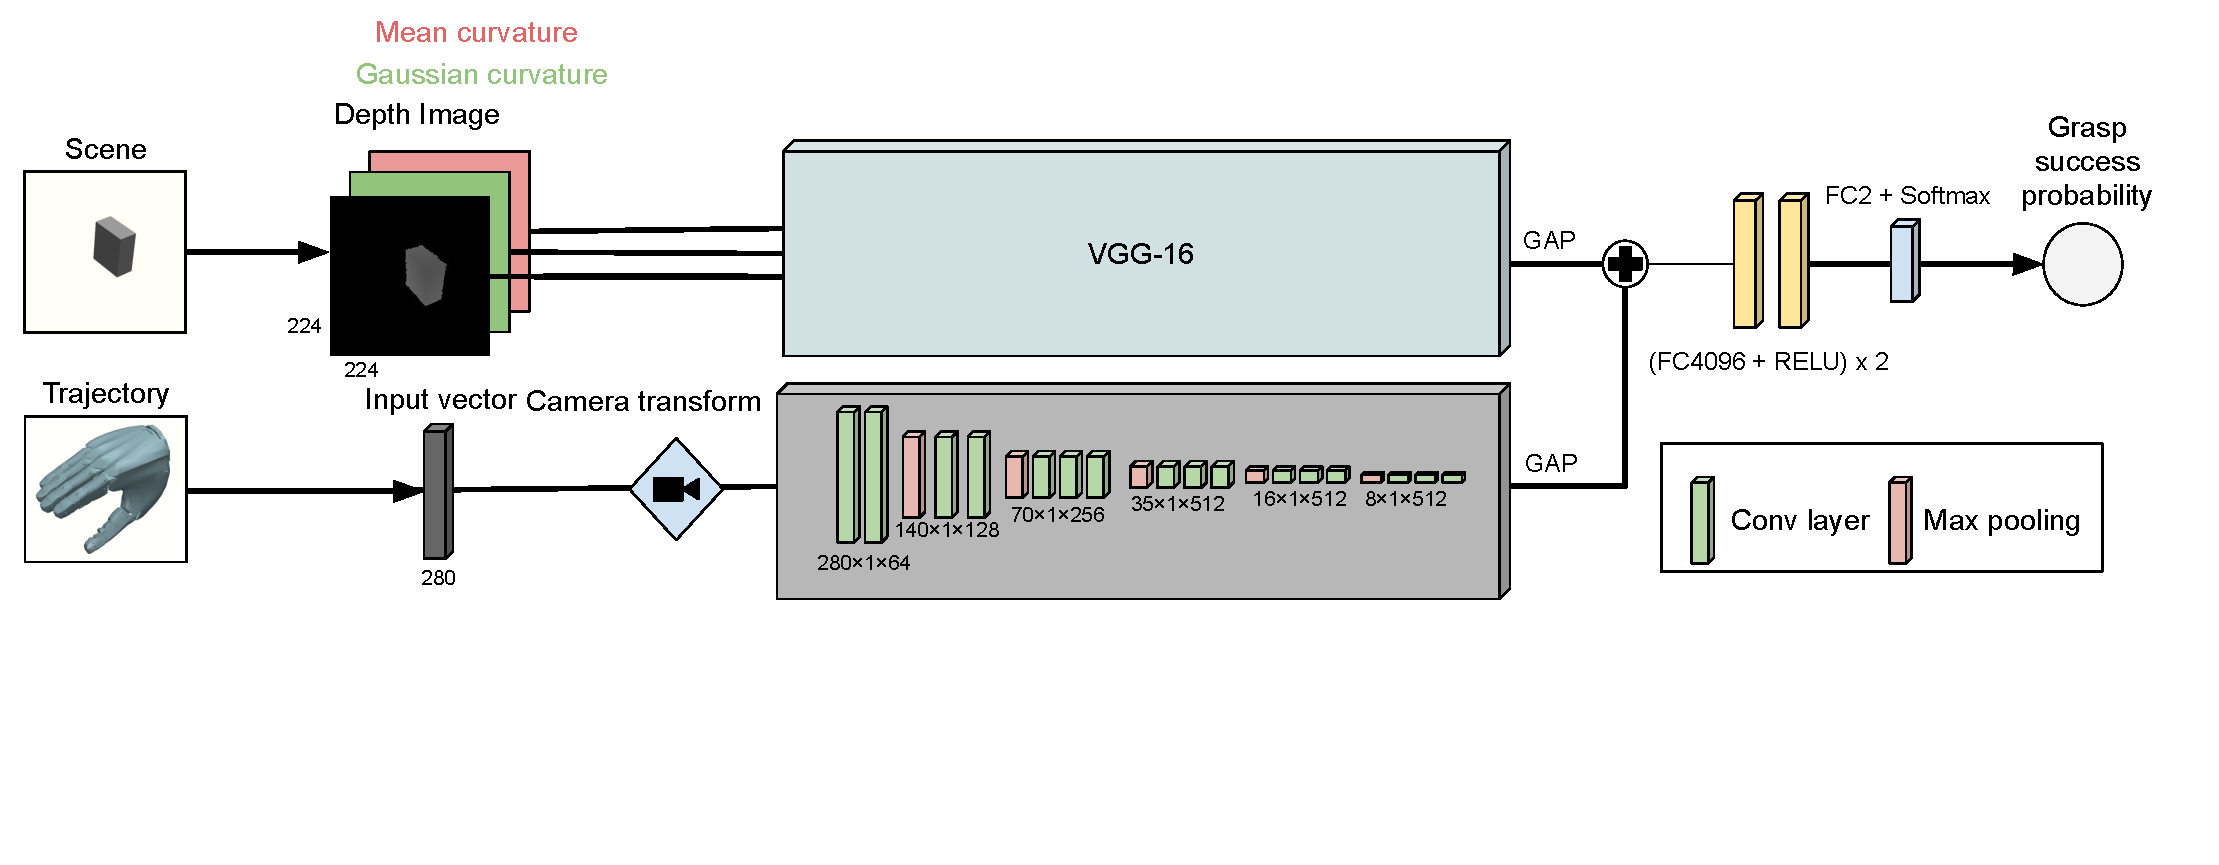
\includegraphics[width=0.8\textwidth]{images/Chaonet_newpic.pdf}
}
% \end{center}

\caption{The three evaluative network architectures presented in this paper. Similar to \cite{Levine1}, the two channels of information (visual data and grasp parameters) are processed in parallel and combined to reach the final decision in each model. RELU activations are used throughout the models, except for the final softmax layers. A final softmax layer has grasp success and and failure nodes, and learns to predict the success probability of a grasp. (a) A VGG-16 based model, where the first 13 convolutional layers of VGG-16 are frozen. (b) ResNet50-based \cite{HeZRS15} network. The first four blocks are used for feature extraction, and the rest of the network is used to learn joint features. (c) Second model based on the VGG-16 architecture. In EM3, the information pathways are joined via concatenation, not addition.
\label{fig:networkArchitecture2}}
\end{figure*}

\subsection{Evaluative Model 1 (EM1)}

Figure~\ref{fig:networkArchitecture2} (a) shows the architecture of the first proposed evaluative network. The colourised depth image is processed with the VGG-16 network \cite{Simonyan14c} to obtain the high-level image features. The VGG-16 network is initialised with the weights obtained from ImageNet training. Only the last three convolutional layers are trained, and the first 13 layers remain frozen. This decision was made in order to speed up training and reduce overfitting.

The grasp parameters and image features pass through fully-connected layers with 1024 hidden nodes (FC-1024) layers in order to obtain two feature vectors of length 1024. The features are combined using the element-wise addition operation, and are further processed using 4 FC-1024 layers. Similarly with \cite{Levine1}, the features are combined using addition and not concatenation. This follows the observation that addition yielded a marginally better performance in the experiments. Furthermore, concatenation and addition can be considered as interchangeable operations when combining different information pathways in deep networks \cite{dumoulin2018feature-wise}. The final FC-1024 layers form the associations between the visual features and hand parameters, and contain most of the trainable parameters in the network. 

\subsection{Evaluative Model 2 (EM2)}

% \begin{figure}[!ht]
%   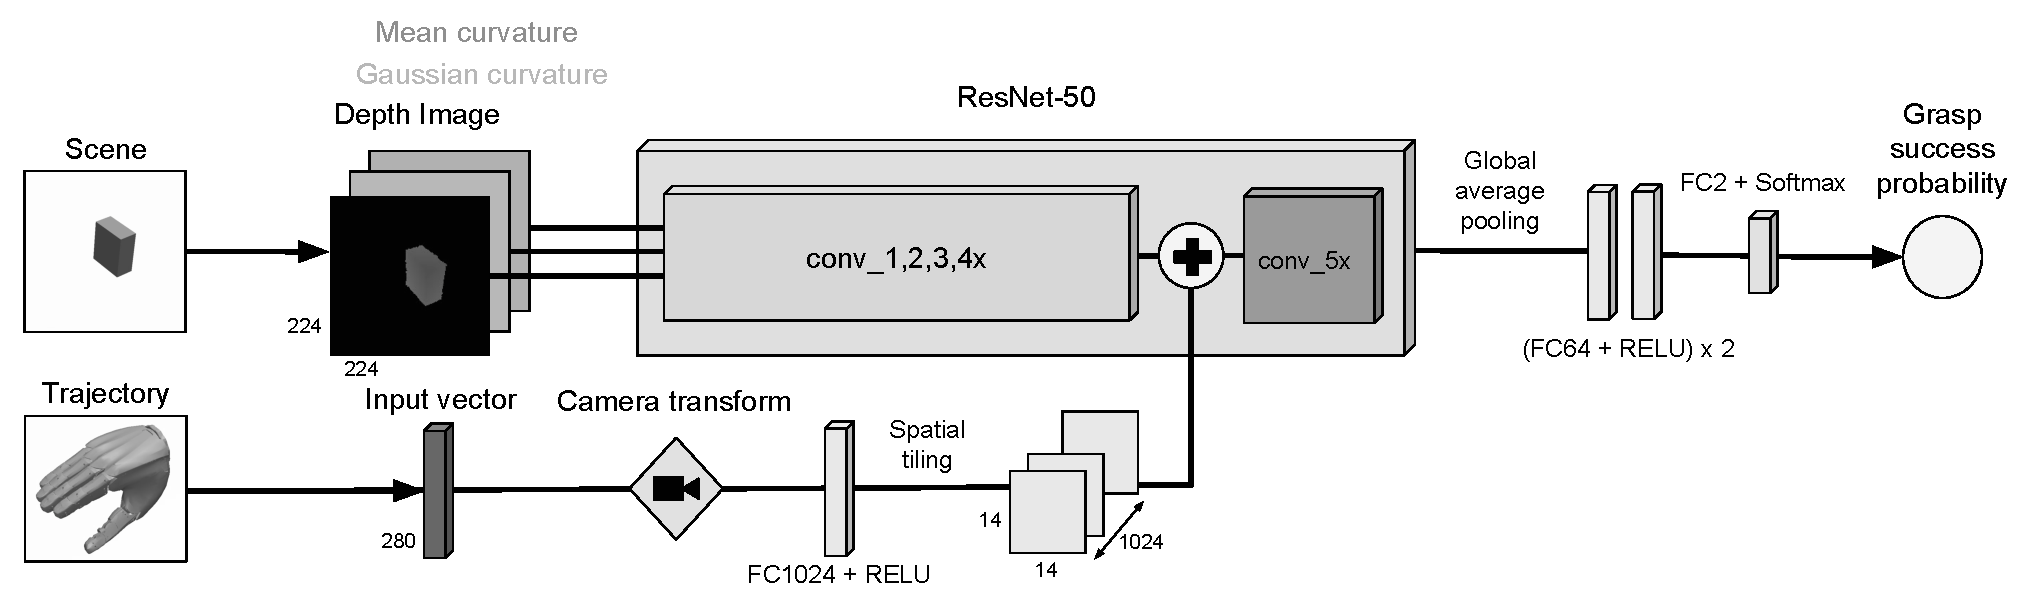
\includegraphics[width=\textwidth]{images/ResNet.pdf}
%   \caption[The ResNet-based evaluative deep neural network architecture.]{The ResNet-based evaluative deep neural network architecture (EM2). Spatial tiling is used to repeat the grasp parameters before they join the image processing pathway. This network requires fewer FC layers due to the earlier marriage of information channels.}
% \label{fig:ResNet}
% \end{figure}

The second evaluative model, termed EM2 (Figure~\ref{fig:networkArchitecture2} (b)), uses the ResNet-50 network in order to obtain the high-level image features. The ResNet-50 architecture is initialised with the weights obtained from ImageNet training. One exception is the last convolution block conv\_5x, which is initialised randomly. In the EM2 architecture, ResNet-50 network is broken down into two parts: the first 4 convolutional blocks are used to extract the visual features. The final convolutional block, which has 9 convolutional layers, combines the image features and grasp parameters. Similarly with EM1, element-wise addition joins the two channels of information. Spatial tiling is used to convert the processed grasp parameters, a vector of size $1024$, to a matrix of size $14 \times 14 \times 1024$. Because the last convolutional block conv\_5x processes combined information, this network is designed with only 2 FC layers with 64 hidden nodes each. The output layer is the same as EM1. 

\subsection{Evaluative Model 3 (EM3)}

This model, similar to EM1 (Figure~\ref{fig:networkArchitecture2} (c)), uses VGG-16 as the base visual model. All 16 layers of VGG-16 are trained. The hand trajectory parameters pass through a feature extraction network before being concatenated with the visual features. Two fully connected layers of higher capacity than EM1-2, contain 4096 hidden nodes each and join the two pathways. A final 2-node FC layer with softmax activation is added to obtain the final decision.

EM3, contrary to EM1 and EM2, uses convolutional layers for feature extraction when processing input grasp trajectories. The trajectory processing pathway is identical to the VGG-16 architecture in that it contains 5 blocks, consisting of a total 13 convolutional layers. The sizes under the blocks are input dimensions. Global Average Pooling (GAP) is performed to obtain 512 features coming from both sides, and they are concatenated to get the combined feature vector of 1024, which further runs through two FC-2048 layers.

All models were trained and tested on simulated data. In addition, EM2 and EM3 were tested on the real robot setup. The next section focuses on the collection of the training data.

\subsection{EM training methodology}
Variants V3-V5 were trained using DS1-Tr. Variants V6-V17 were trained using the combined data set from DS1-Tr and DS2-Tr. The ADAM optimiser was employed with starting learning rate of 0.01, a dropout rate of 0.3, and early stopping. We halve the learning rate every 5 epochs during training.

\subsection{Grasp optimisation using the EM}

So far we have considered only Generative-Evaluative architectures where the Evaluative Model merely ranks the grasp proposals. As proposed by Lu et al. \cite{lu2017planning} we may also use the EM to improve grasp proposals. This boils down to searching the grasp space driven by the EM as the objective function. This may be by gradient descent or simulated annealing. The methods V12-17 use V8 as the objective function, hence V8 should be treated as the baseline. We employed both gradient descent based optimisation and simulated annealing.

\subsubsection{Gradient based optimisation}
Lu et al. \cite{lu2017planning} proposed gradient ascent, modifying the grasp parameters input to the EM with respect to the output predicted success probability. They initialised with a heuristically selected pre-grasp. We initialise with the highest ranked grasp according to the EM. We investigated three variants:
\begin{itemize}
\item GD1: Shifts the position of the all waypoints in the grasp trajectory equally. The gradient is the average gradient of the EM output across all 10 waypoints
\item GD2: Tunes the hand configuration by tuning the angle of each finger joint. Every finger joint at each waypoint is treated independently.
\item GD3: Performs GD1 and GD2 simultaneously.
\end{itemize}

\subsubsection{Simulated annealing based optimisation}
Gradient based optimisation is sensitive to the quality of gradient estimates derived from the model. Simulated annealing (SA) based optimisation is more robust to such noise. Therefore, three optimisation routines were implemented using SA:
\begin{itemize}
\item SA1: Shifts the position of the all waypoints in the grasp trajectory equally. Moves are drawn from a three-dimensional Gaussian noise vector, with $\mu=0$ and $\sigma=0.001$. 
\item SA2: Perturbs the finger joints along the entire trajectory. The pose of all joints in a finger with respect to a reference pose (fully open hand) is modified jointly, which results in exploration of how open or closed the hand is. The opening/closing ratio for each finger is determined by a noise vector that is drawn from a Gaussian distribution with $\mu=0$ and $\sigma=0.01$. 
\item SA3: Performs SA1 and SA2 simultaneously.
\end{itemize}